\chapter{Events}
\section{Types of Events}
\section{Anatomy of an Event}
\begin{center}
	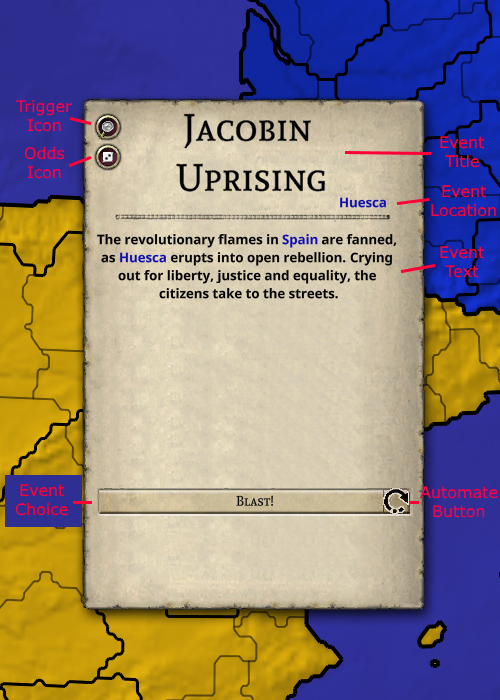
\includegraphics{province_event.png}
	\small{a typical province event}
\end{center}
\subsection{Trigger Icon}
An explanations of the conditions that allow the event to occur appear when the cursor is over the trigger icon.

\begin{center}
	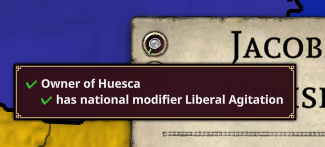
\includegraphics{province_e_trigger.png}
\end{center}

A green check mark indicates a part of the condition that is currently met, while a red x shows any parts of the condition that are not currently satisfied. An event that is not explicitly triggered by another event or a decision will not appear if the necessary condition is not met, regardless of what the odds are.
\subsection{Odds Icon}
An explanation of the monthly probability that the event will occur appears when the cursor is over the odds icon.

\begin{center}
	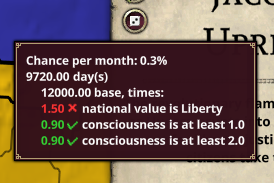
\includegraphics{province_odds.png}
\end{center}

The first line displays the currently monthly chance that the event will trigger. For a province event, this is the chance for each province that meets the necessary conditions, while country events are checked only once per nation. The next line contains the effective ``days'' value after any applicable modifiers have been applied. The exact relationship of this value to the event's probability is detailed below; for now it suffices to say that events with a lower ``days'' value are more likely to occur. The line after that contains the base ``days'' value, followed by any modifiers that could apply to it. Each potential modifier is displayed as a red or green value followed by the conditions under which that modifier may apply. If the modifier currently applies its condition will have a green check mark next to it; if the modifier does not apply a red x will appear instead. Each of these modifier is multiplied with the base ``days'' value to obtain the final result. Thus modifiers less than 1 make the event more likely to occur (and their values are displayed in green) while modifiers greater than 1 make the event less likely to occur (and their values are displayed in red).
\subsection{Event Title and Text}
The event title and text do not have any game mechanical effects. However, any blue text will function as a link. Clicking on this text will move the camera to the entity described and open either the appropriate province or diplomacy window.
\subsection{Event Choices}
At the bottom of each event are one or more buttons, each representing a single possible response to the event.

\begin{center}
	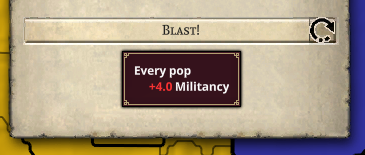
\includegraphics{province_e_button.png}
\end{center}

Moving the mouse over each of the buttons reveals the game effects of choosing that option. Unless stated otherwise, the effects apply only to the province the event has occurred in, for province events, or to the nation it has occured in, for country events.
\subsection{Event Automation}
If it is possible for the particular event to occur more than once in a single game, then an additional automation button will appear to the right of every choice button.

\begin{center}
	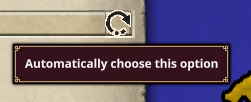
\includegraphics{province_e_automate.png}
\end{center}

Clicking on this button will choose that option for the event and will also cause that option to be chosen automatically any time the event occurs in the future for you. Such events will no longer pause the game or be displayed. Instead, you will receive a message that the event has occurred, either with a pop up or by an entry in the log, depending on your message settings. Event automation choices are specific to each save file: they do not carry over from one game to the next.

\section{Event Probabilities}
The events are divided into 32 ``buckets'' and each day the events belonging to one of those buckets is checked. The probability a province event will occur on a day it is checked for, assuming its conditions are met, is:
	\[
	1 - \left( 1 - \frac{2}{d} \right)^{16}
\]
where \( d \) is the modified ``days'' value. A country event on the other hand, has a probability of:
\[
	1 - \left( 1 - \frac{1}{d} \right)^{16}
\]
in other words, less than the same ``days'' value would yield for a province event.

This method of determining whether an event occurs differs from that of the base game in some of its details. The base game checks the conditions of all of the events once per month. Those events with conditions that are satisfied go into a pool. Then, on alternating, days either the province events or the country events. If its conditions are still met, the events have a probability of \( 2/d \) for province events or \( 1/d \) for country events. Although the details differ, the effect of the two systems is much the same. First, in both there is a period of up to a month between when the conditions for an event are first met and when it can first fire. Secondly, there is the same chance in a 32 day period of seeing a particular event at least once, assuming the condition for it occurring remains satisfied and the modified ``days'' value remains constant.

Finally, a note on ``days.'' I continue to use this term because it is directly derived from the way the events are described in the text files that generate the scenario. The modifiers that affect an event's probability are typically described as modifiers to the mean time to happen, the base value of which is a number of days, months, or years (months and years becoming the appropriate number of days internally). Despite this description, it is true neither in Open V2, nor in the base game, that on average an event will occur 50\% of the time in that many days.